\documentclass[a4paper]{article}
\usepackage{ctex}
\usepackage{graphicx}
\title{毕设报告}
\author{辛文钧}
\begin{document}
	\maketitle
	\section{识别部分}
	\begin{itemize}
		\item 读取机器人摄像头数据,采集障碍物图片(虚拟环境中我把障碍物定为书架)
		\begin{figure}
			\centering
			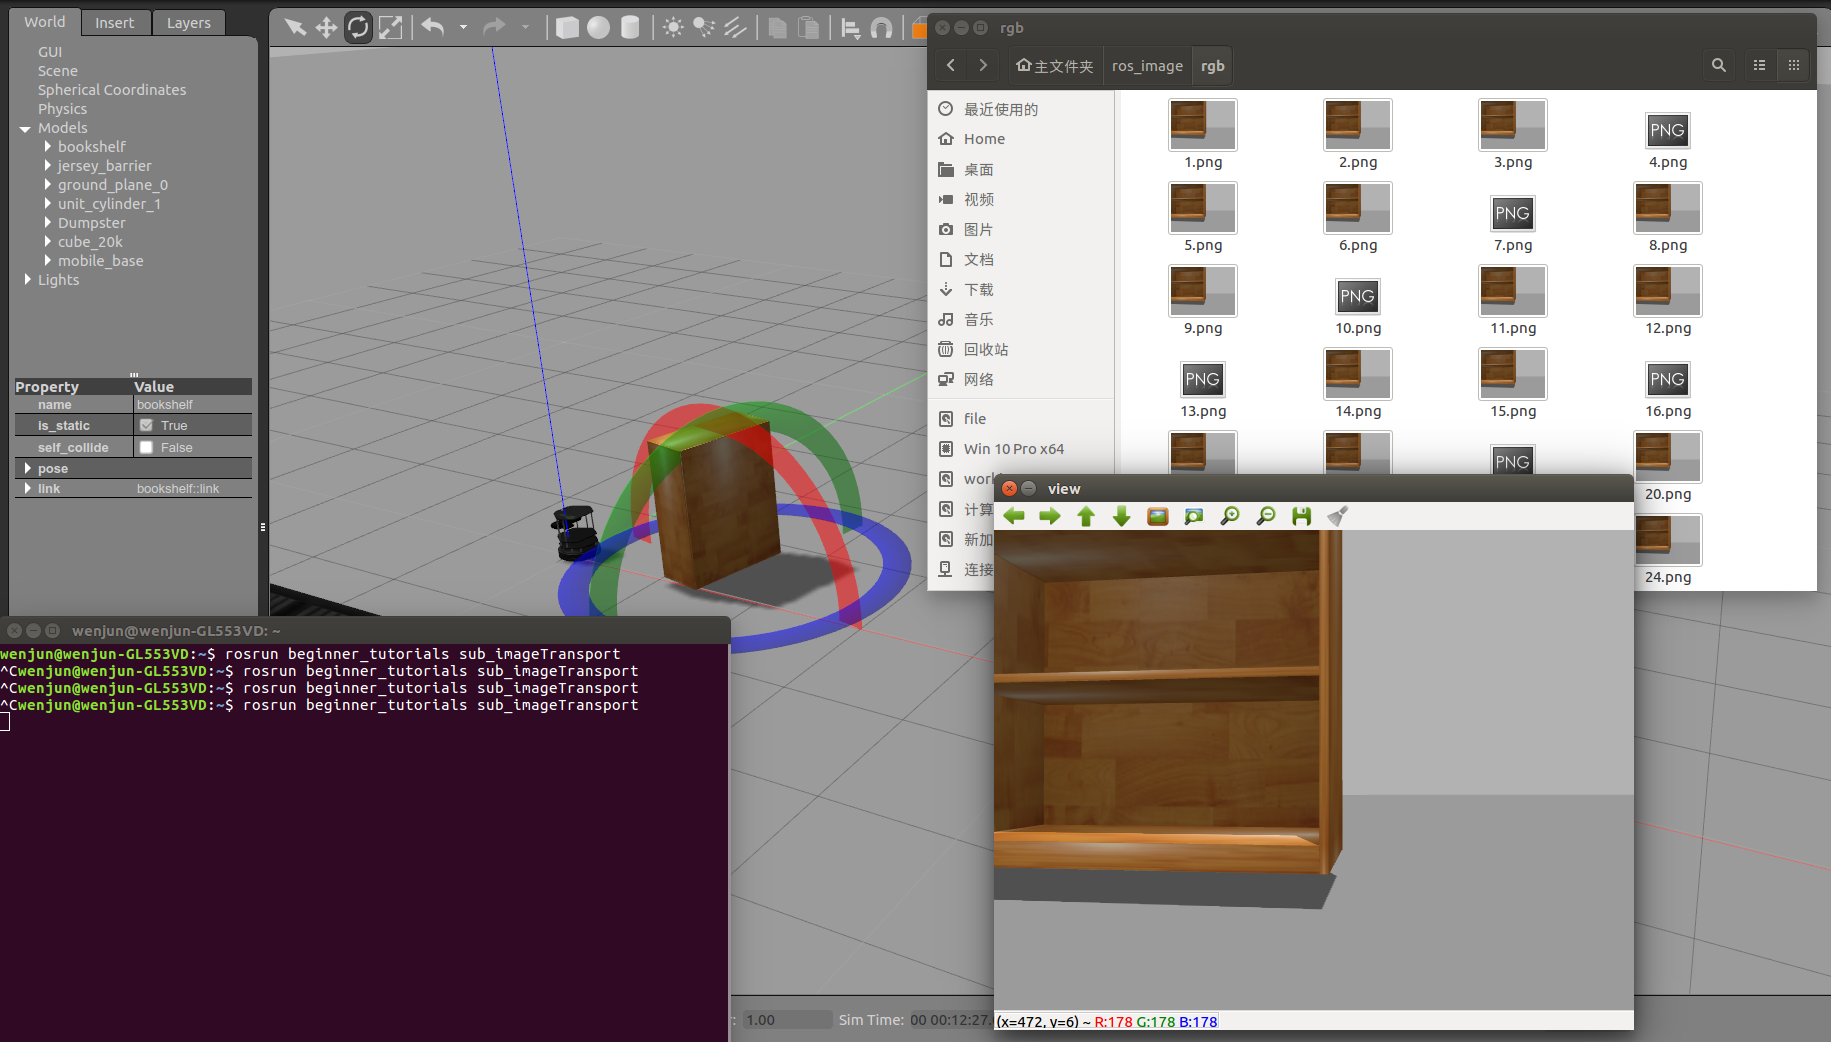
\includegraphics[scale=0.25]{sample.png}
			\caption{采集图片}
		\end{figure}
		
		\item 学习卷积神经网络
	\end{itemize}
	\section{强化学习}
	学习DDPG算法,在查找相关论文时找到一份《基于深度强化学习的机器人导航研究》,他用的方法也是DDPG算法,并且环境相同,但是是通过雷达识别障碍物,状态空间和动作空间大体相同,我觉得可以参考一下他的想法。
\end{document}